\documentclass[../main.tex]{subfiles}
\begin{document}

\chapter{Preventing unauthorized access}

\section{Introduction}
\subsection{Access control in web applications}
\begin{itemize}
\item Authentication is only the first step
\item Authentication in web applications is one of these topics with a long history. Everybody has their idea of how to do it, and most of these ideas are antiquated.
\item Also storing credentials is harder then you would think.
\item Using multi-factor authentication also provides several benefits.
\item Many applications keep track of the user's authenticated state in a session object. Sadly most of them fail to get the details of secure session management right.
\item On the one hand, the application needs to enforce proper permissions on access to data or operations. But on the other hand, the application also needs to ensure that actions carried out in the user's name are intentional.
\end{itemize}

\subsection{Introducing state into your application}
\begin{itemize}
\item HTTP is a stateless protocol $\rightarrow$ authentication and authorization are challenging.
\item \textbf{HTTP Basic Authentication}
\begin{enumerate}
\item Server tells browers that a resource is off limits.
\item Browser will prompt the user to authenticate.
\item With the user's credentials, the browser again tries to fetch the resource. The credentials are present in the Authorization header.
\item The server can now verify the credentials and decide if the user can access the resource. If the answer is affirmative, the response has \textbf{status code 200} and contains the resource. Otherwise, the server can send an error message with \textbf{status code 403}.
\end{enumerate}
\item Note that the Authorization header does not contain the cleartext credentials. The browser has \textbf{base64-encoded} them to ensure they can be safely used in an HTTP message $\rightarrow$ can easily be undone, not for security reasons. Because it is sent as part of the request, and passwords can contain any kind of characters. Some of these characters could confuse the server parsing the headers, resulting in vulnerabilities.
\item Drawbacks:
\begin{enumerate}
\item it provides only the identity of the user $\rightarrow$ no support to track additional properties
\item The username and password are present in every request $\rightarrow$ All an eavesdropper needs to impersonate the user is to capture one request.
\item Once entered by the user, the browser keeps using the credentials for that website. The only effective way for the user to log out is to close the browser.
\item The browser handles authentication in a popup window. As a consequence, the authentication form cannot be integrated into the application's UI.
\end{enumerate}
\item Today, most applications use a custom authentication form, in combination with session management.
\item Session management ensures the propagation of authentication information.
\item Unfortunately, this complex configuration is prone to mistakes and misconfigurations. Many applications suffer from broken authentication and session management. These issues are quite severe, as they result in unauthorized access to the application. The OWASP top 10 even ranks them in second place.
\end{itemize}

\section{Secure authentication}
\subsubsection{The truth about passwords}
\begin{itemize}
\item More and more voices are proclaiming passwords as insecure, inefficient or even outright evil. They advocate the use of alternative authentication mechanisms, such as hardware tokens or mobile applications. $\rightarrow$ but complicated and disruptive.
\item Almost every application today still uses passwords.
\item One of the weakest security properties of a password is that it is usable by anybody that knows it.
\item Various kinds of attacks.
\begin{itemize}
\item Guess the password, using a variety of techniques (using personal information, dictionary attacks, lists of commonly used passwords,...)
\item \textbf{phishing attack}: tricks the user into visiting a malicious website. This website looks exactly like an innocent one. When the user authenticates to the malicious site, the attacker steals the user’s credentials.
\item Hacking the application and stealing the database $\rightarrow$ many applications store passwords in an insecure way.
\end{itemize}
\item These attacks are amplified by the fact that many people reuse passwords across accounts. Everyone has dozens of accounts with a password, and remembering a unique password for each account is next to impossible. As a result, obtaining a single password gives the attacker access to many accounts of the same user. The increase in data breaches has resulted in massive online dumps of credentials.
\item The problem is so bad that there is even a website keeping track of all the accounts in the data dumps. The site is \textbf{Have I Been Pwnd}, and it allows you to see if your email address occurs anywhere in the set of data dumps.
\item The best way to improve the security of passwords is by using a \textbf{password manager}. A password manager is an application that securely stores credentials for various accounts. The biggest benefit is that the user no longer needs to remember them. As a result, password managers enable the use of a unique and complex password for every account.
\item Eliminates security problems.
\begin{enumerate}
\item Guessing attacks become irrelevant, since passwords can now be long and random.
\item There is no longer a need reuse passwords across accounts.
\item Increase the resilience against phishing attacks. Many password managers offer autocomplete features in the browser. But in a phishing attack, the URL points to a malicious site, so the password manager will not find any associated accounts.
\end{enumerate}
\item If you don't want to use a password manager, you can take some countermeasures as well (e.g. divide accounts into trust levels, and use a different password for each of these levels).
\end{itemize}

\subsubsection{Insecure password storage}
\begin{itemize}
\item One of these weak behaviour patterns is reusing passwords across many applications.
\item It is best to adhere to a defense-in-depth strategy to minimize the impact of a data breach $\rightarrow$ Store your passwords securely!
\begin{enumerate}
\item \textbf{Plain text}: problematic in light of a data breach, attacker has full access. 
\item \textbf{Hashed (MD5,SHA1...)}: two users pick same password $\rightarrow$ same hash + \textbf{rainbow tables}: tables of precomputed hashes of commonly used passwords $\rightarrow$ retrieving passwords from the stolen data becomes trivial.
\item \textbf{Hashed with salt}: long, random string per user, that is appended to the password before it is hashed. The application stores the salt in the database, alongside the hash of the password. During authentication, the application recomputes the hash with the plaintext password and the salt. If the hash matches the stored hash, the user has provided the original password $\rightarrow$ precomputation attacks are infeasible.\\
\emph{But:} It is weaker than you might expect. Hashing algorithms are designed to be fast $\rightarrow$ brute force attack to try out each of the passwords with all the salts. This approach is not infeasible using modern-day GPU-based password cracking software.
\end{enumerate}
\end{itemize}

\subsubsection{Secure password storage}
\begin{itemize}
\item To prevent brute force attacks, you should use a dedicated password hashing function. These are cryptographic functions that perform a certain amount of iterations to calculate the output. As a result, they are expensive to execute, and withstand brute force attacks by design. In practice, all recommended password hashing functions also use a salt to ensure that even if two users pick the same password, the hash will be different.
\item Popular dedicated password hashing functions: \textbf{bcrypt, argon2, PBKDF2, scrypt...}
\item The output of the bcrypt function contains several parts: 
\begin{enumerate}
\item The first part indicates which algorithm has generated the hash.
\item The second part specifies a \textbf{cost parameter} (makes the function more expensive to execute).
\item The third part contains a salt and the resulting hash.
\end{enumerate} 
\item For a cost factor of 5, a very powerful machine (8 Nvidia GTX GPUs) can only calculate 100 000 hashes per second.
\begin{figure}[h!]
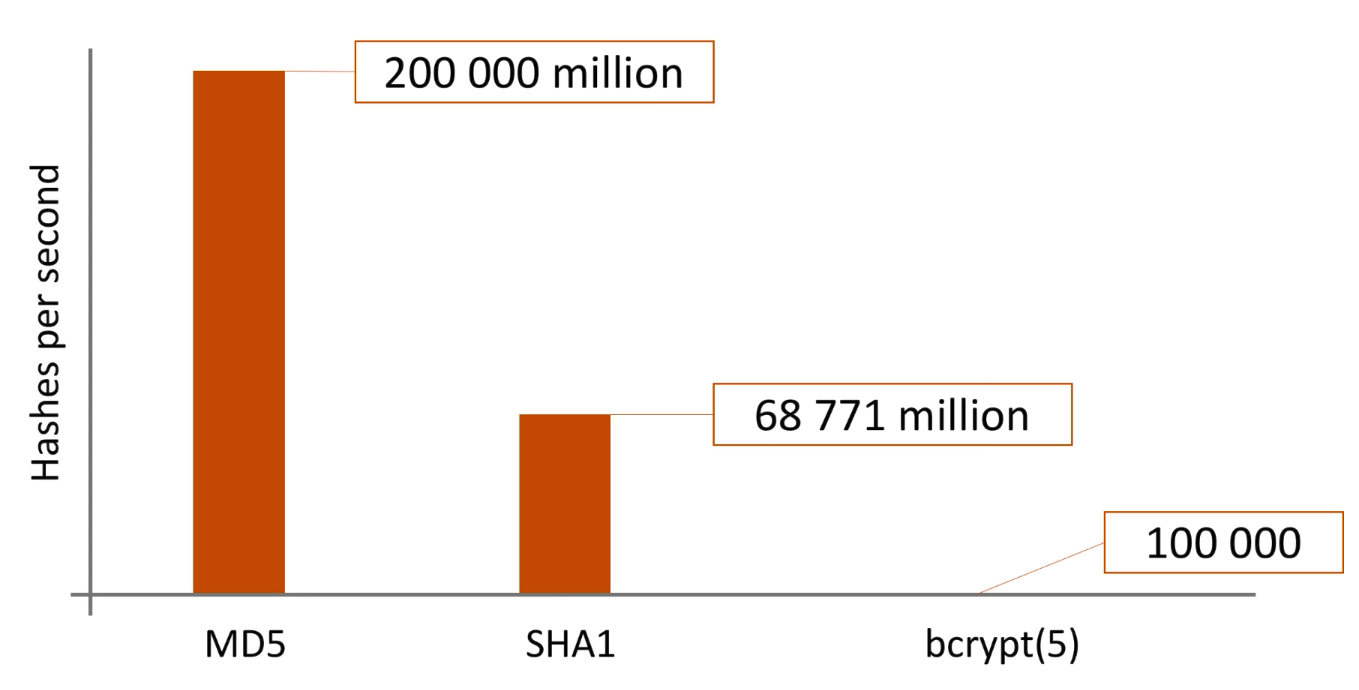
\includegraphics[width=\textwidth]{../images/bcrypt}
\caption{Comparison between MD5, SHA1 and bcrypt (cost factor 5) on system with 8 Nvidia GTX GPUs}
\end{figure}
\item Note that the cost factor is exponential and that the current recommendations list 12 as a minimum.
\item There are a few strategies you can follow to upgrade the storage mechanism.
\begin{enumerate}
\item \textbf{Gradual upgrade path}: When the user has provided a valid password, the application checks how the password is stored in the database. When the stored hash is calculated with a legacy algorithm, it needs to be updated. The application uses the password to calculate a bcrypt hash, and stores the new hash in the database. Running this gradual upgrade strategy for a couple of months will replace the stored hashes for all your active users. At a certain point in time, it makes sense to reset the passwords on all accounts that have not yet been upgraded. If users want to resume their account, they can use the account recovery process.
\item \textbf{Drastic update}: Imagine that you have a database full of unsalted MD5 hashes. If you want to upgrade your application to bcrypt, you can use the MD5 hashes as input for the bcrypt function. The database now contains bcrypt hashes of MD5 hashes of the plaintext password. For the authentication procedure you first have to check the validity of the provided password by double hashing it. Next, you use the plaintext password to calculate a single bcrypt hash and replace the double hash with the newly generated one.
\end{enumerate}
\end{itemize}

\subsubsection{Preventing enumeration attacks}
\begin{itemize}
\item In a \textbf{brute force attack}, the attacker tries to guess the password of a valid user of the application $\rightarrow$ can be very effective!
\item With an \textbf{enumeration attack}, the attacker can determine if a username exists in the application. If the application leaks such information, it can be abused to compile a list of valid usernames. That list, in turn, enables the attacker to optimize his brute force attack.
\item Where does an application leak usernames?
\begin{enumerate}
\item \textbf{Authentication forms}: Don't choose an error message that reveals whether a username exists or not.\\
\emph{Fix:} Avoid leaking information about the existence of an account.
\item \textbf{Account recovery form}: More often than not, it immediately notifies the user when the email address is not found.\\
\emph{Fix:} The first step is to refrain from giving the user immediate feedback about the existence of an email address. Instead, you look up if an email address exists. If it exists, you send the recovery email, like before. If it does not exist, you can send a message that informs the user about the potential account recovery. You can point out that the user may have used a different email address to sign up. Alternatively, you can suggest that the user can always register a new account if desired.
\item \textbf{registration form}: When choosing a username or email address, the application discloses if it already exists.\\
\emph{Fix:} The simple case is when the application uses email addresses as a unique identifier. In this case, you can implement a similar mechanism as for recovery. If the email address is not yet known to the application, you create a new account and send an email to the user. If the email address matches an existing account, you send an email to remind the user of this account. You should also include instructions on how to recover the password. Things become a lot more complicated if the application uses arbitrary identifiers, such as usernames. The application will have to enforce uniqueness across the entire userbase. However, these identifiers are chosen by the user. One way to limit this risk is to require registration with an email address first. Only then allow the selection of a username. This allows you to impose a limit on the number of attempts to pick a username. As a result, the attacker can only learn a tiny amount of information during an attack.
\end{enumerate}
\item There are two common strategies to prevent brute force attacks.
\begin{enumerate}
\item Lock a user account after a certain number of authentication attempts $\rightarrow$ How will you distinguish a forgetful user from an attacker? Will you need to manually intervene to unlock an account? What happens if an attacker locks all accounts in your application?
\item Slow down authentication attempts after a couple of failures $\rightarrow$ increasing the slowdown makes a brute force attack infeasible.
\end{enumerate}
\end{itemize}

\subsubsection{Beyond password-based authentication}
\begin{itemize}
\item Passwords are a weak form of authentication $\rightarrow$ other means of authentication exist as well (possession of a physical device, biometrics, behavior and context...).
\item \textbf{Multi-factor authentication}: Using an alternative authentication method in combination with a knowledge-based authentication.
\item E.g. The combination of a username and password with an SMS-based verification code.
\begin{itemize}
\item The user links a mobile phone number with his account. When the user logs in, the application sends a random verification code to the phone number. The user enters this code into the second login form, and the application compares if the codes match.
\item At first sight, an SMS-based verification code seems very secure.
\item But because this scheme makes a lot of assumptions, it suffers from a variety of weaknesses.
\begin{enumerate}
\item If the user stores his password on his smartphone, the attacker only needs to access the phone.
\item An attacker setting up a phishing site can still trick the user.
\item If the attacker can take control of the phone number, he can receive the verification code (tricking phone company or abusing the underlying cellular protocols).
\end{enumerate}
\item No longer recommended to use a mobile phone number as an authentication factor.
\end{itemize}
\item E.g. The use of a U2F security key.
\begin{itemize}
\item \textbf{U2F} stands for \textbf{Universal Second Factor}, and is an open standard for device-based authentication on the web (e.g. \textbf{Yubikey}).
\item Supported by numerous major application providers, including Google and Facebook.
\item To use a U2F device, the user first registers it with his account. From then on, the second step in the authentication process is inserting the U2F key and touching the device. The device will use an embedded secret to sign a challenge, proving to the application that it is the same device as registered before. Multi-factor authentication with U2F devices is a secure scenario. The successful signing of a challenge indicates the possession of a previously registered key. The touching of the U2F device indicates a physical presence of the user. This step makes it much harder for malware to trick the device into signing a challenge. Additionally, the origin of the context where the authentication happens is part of the signature. 
\item Not susceptible to phishing.
\end{itemize}
\item But companies such as Google and Facebook have already implemented all of this, and probably better than you ever can. Why not use this? $\rightarrow$ outsourcing of authentication to third parties (\textbf{social login}).
\item Under the hood, delegating authentication often depends on the use of \textbf{OAuth 2.0} or \textbf{OpenID Connect}.
\begin{enumerate}
\item When the user opts for a social login, the application redirects the user to the third-party authentication provider.
\item If the user is not logged in, the provider will trigger its own authentication procedure.
\item Once authenticated, the provider verifies whether the user allows the use of social login for our application. When allowed, the authentication provider redirects the flow back to our application, and passes a security token as part of the URL.
\item With this token, our application can request information about the user from the provider. This information allows our application to identify the user.
\end{enumerate}
\item Implementing multi-factor authentication a considered a best practice today, but it requires a significant amount of effort. A good alternative is delegating authentication to third-party providers.
\item Implementing this in practice poses many challenges, and lots of insecure implementations exist!
\end{itemize}

\end{document}